%=============================--A--=============================%
\subsection{Módulo 3 $\pmb \mapsto$ Recuperaç\~ao da componente stereo $(L - R)$}
\label{subsec:mod3}

%\iffalse
\begin{figure}[H]
    \centering
    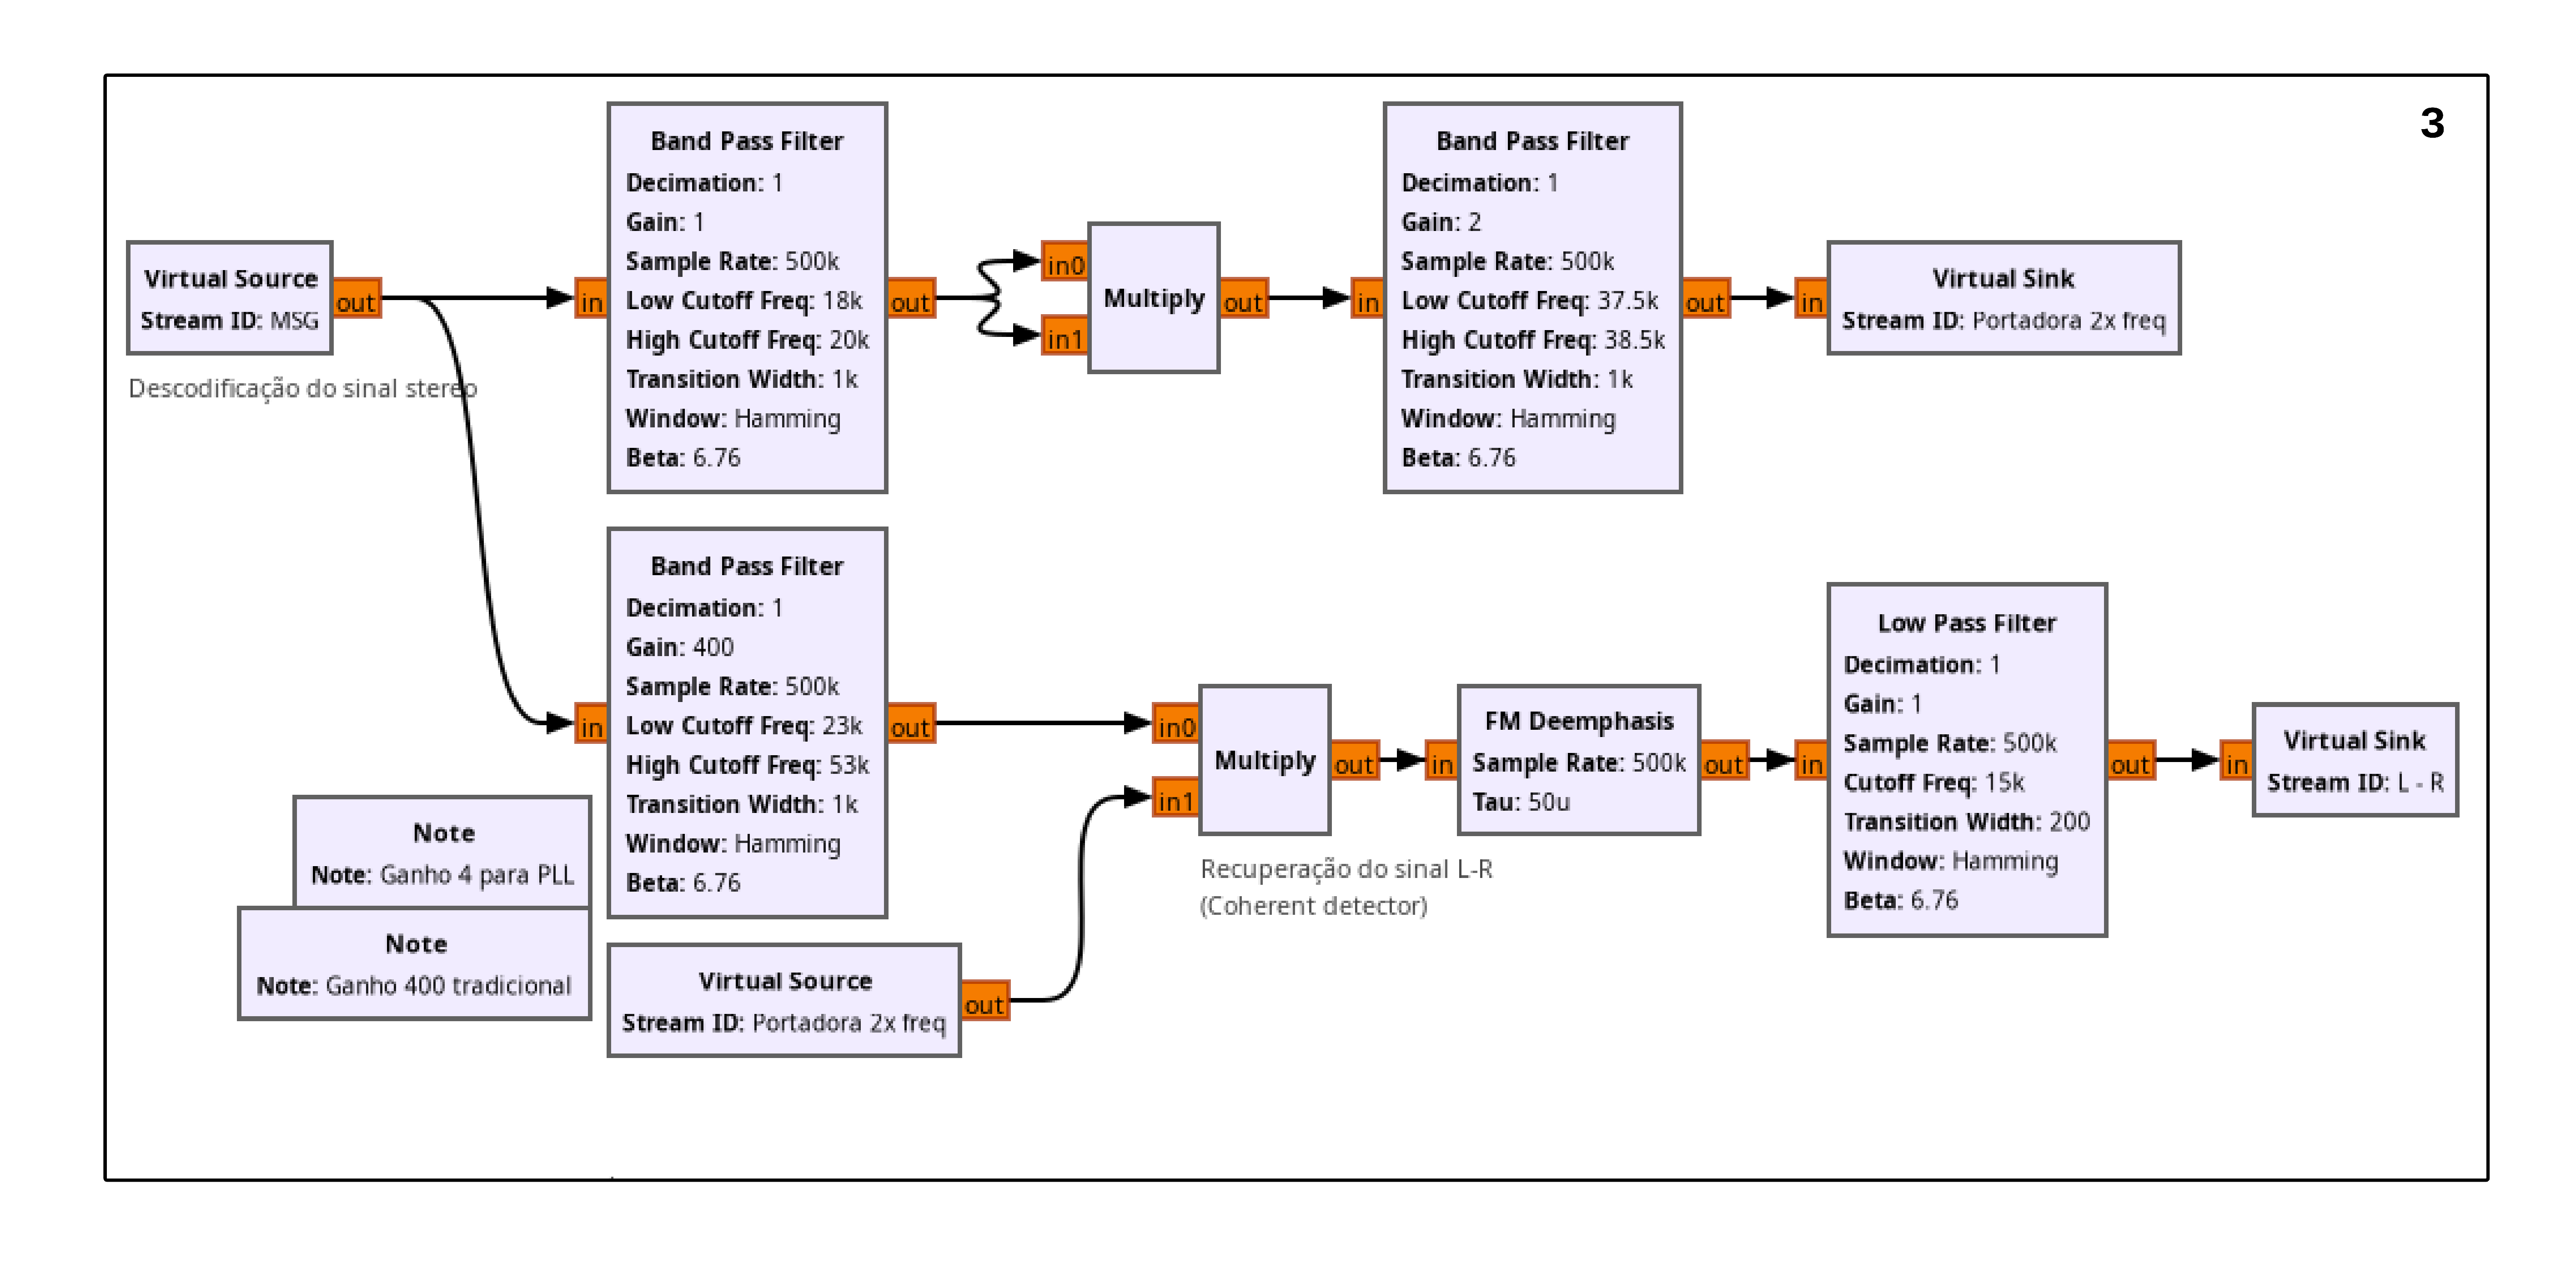
\includegraphics[width = \linewidth]{img/mods/modulo3.png}
    \caption{Recuperação da componente estereofónica da mensagem.}
    \label{fig:modulo3}
\end{figure}
%\fi

Este \hyperref[subsec:mod3]{módulo} pode ser visto em dois momentos: 
\begin{itemize}
    \item[$\mapsto$] \hyperref[subsubsec:regen]{Regeneração da subportadora e duplicação da sua frequência} \hyperref[fig:modulo3]{(no ramo superior)}
    \item[$\mapsto$] \hyperref[subsubsec:coherent]{Deteção coerente da DSB-SC $L-R$} \hyperref[fig:modulo3]{(no ramo inferior)}
\end{itemize}
%1
%1
%=============================--B--=============================%
\newpage
\subsubsection{1. Regeneração da subportadora e duplicação da sua frequência}
\label{subsubsec:regen}

A recuperação tradicional da portadora implica a passagem da mensagem por um filtro passa-banda muito fino (\textit{narrow-band}) em torno dos $19\ \text{kHz}$ (vide \hyperref[fig:stereo_spectrum]{Fig. 1}), para a recuperação da subportadora piloto. O posterior processo de duplicação de frequência envolve multiplicar este \textit{output} do filtro por si próprio:
$$\text{Narrow-band BPF $\sim$19 kHz} \implies \text{output :=}\ K \cdot\cos{(2\pi f_c\cdot t)} $$
$$ \text{Portadora 2x freq.}\ =  (K \cdot\cos{(2\pi f_c\cdot t)})^2 =$$
$$ = K^2 \cdot \cos^2{(2\pi f_c\cdot t)} = K^2 \cdot (\frac{1}{2} + \frac{1}{2}\cos{(2\pi (2f_c)\cdot t)})$$

É então aplicado um filtro passa-banda em volta dos $38\ \text{kHz}$, ou, teoricamente, um passa-alto\footnotemark[1], para a destruição da componente DC, com um ganho de 2 (dadas as identidades trigonométricas), e finalmente:
$$ \pmb{\therefore}  \text{\textbf{Portadora 2x freq.}} = K^2\cdot \cos{(2\pi (2f_c)\cdot t)}$$

\footnotetext[1]{No entanto, menos desejável nesta aplicação, já que o foco do passa-alto não é isolar a portadora do ruído, mas sim eliminar a componente estática.}
%2
%2
%=============================--C--=============================%
\subsubsection{2. Deteção coerente da DSB-SC $L-R$}
\label{subsubsec:coherent}

Voltando ao processo de recuperação do sinal $L-R$. Devemos primeiro analisar a \hyperref[fig:modulo3]{Fig. M3}, onde é aparente um ganho de 400 no filtro passa-banda (com frequências de corte de acordo com o espectro da mensagem já mencionado) que isola a componente estereofónica DSB-SC.

A dedução desta constante de correção foi efetuada através de uma análise teórica e prática:

Analisando somente o processo de deteção coerente, obtemos:
$$\text{DSB-SC L-R :=}\ [L-R]\cos{(2\pi (2f_c)\cdot t)}$$
$$\implies (\text{DSB-SC L-R})\cdot (\text{Portadora 2x freq.})=$$
$$= (\text{DSB-SC L-R})\cdot K^2 \cos{(2\pi (2f_c)\cdot t)} =$$
$$= [L-R]\cdot K^2\cos^2{(2\pi (2f_c)\cdot t)} =$$
$$= [L-R]\cdot K^2\left(\frac{1}{2} + \frac{1}{2}\cos{(2\pi (4f_c)\cdot t)}\right) $$

Que após a passagem no filtro passa-baixo final (assumindo ganho unitário em todos os filtros deste ramo, para demonstrar os fatores a compensar):
$$\therefore \text{Sinal $[L-R]$ recuperado por compensar}\ = [L-R]\cdot \frac{K^2}{2}$$

No entanto a prova empírica (exercida com os ficheiros de calibração LEFT e RIGHT) indica que é necessária a correção de um fator multiplicativo extra de 1/2 para que os sinais $L+R$ e $L-R$ possuam a mesma amplitude, de modo a que seja possível proceder ao \hyperref[subsec:mod4]{módulo seguinte} e efetuar a recuperação de $L$ e $R$ de forma bem sucedida.

\newpage

\begin{figure}[ht] 
    \begin{subfigure}[b]{0.5\linewidth}
        \centering
        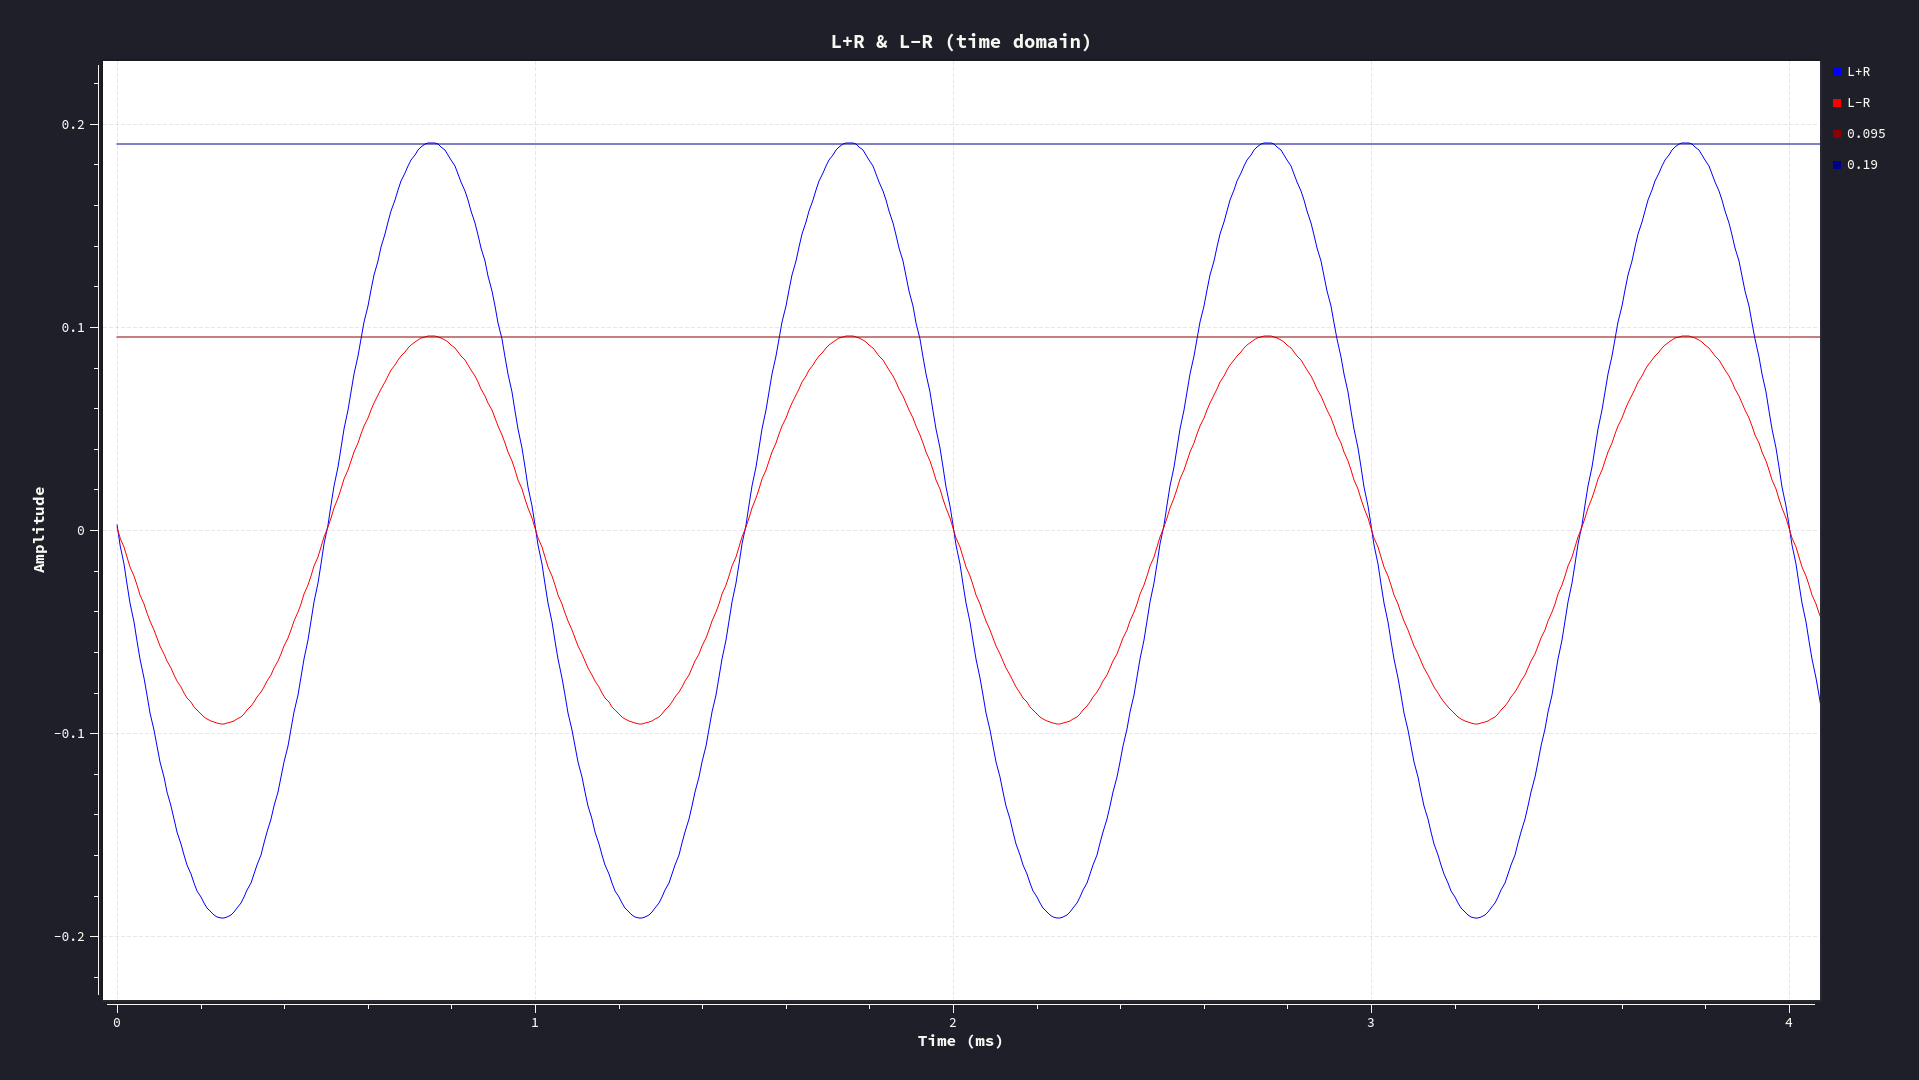
\includegraphics[width=0.8\linewidth]{img/1_2LEFT.png}
        \caption{LEFT: visualização de $L+R$ e $L-R$ (domínio \\ do tempo)} 
        \label{fig:aaa} 
        \vspace{1ex}
    \end{subfigure}%% 
    \begin{subfigure}[b]{0.5\linewidth}
        \centering
        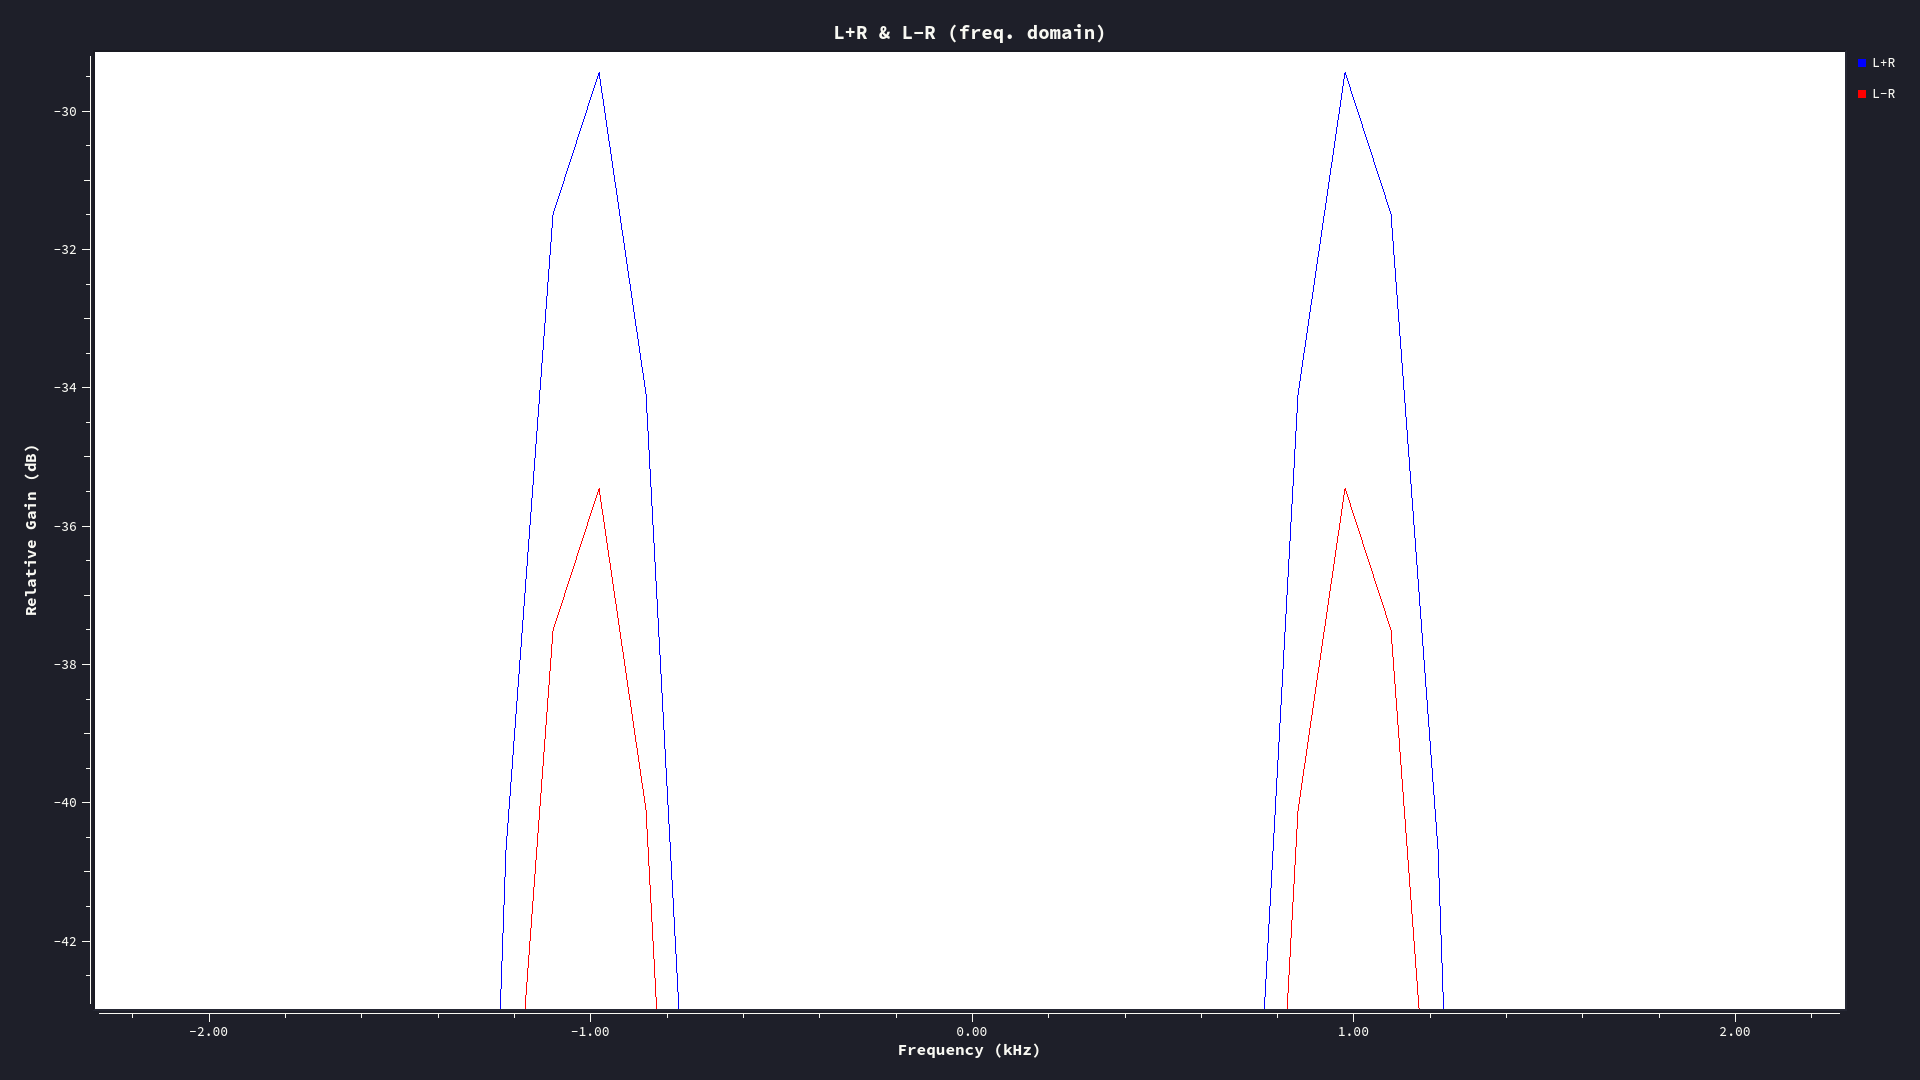
\includegraphics[width=0.8\linewidth]{img/1_2LEFTdB.png} 
        \caption{LEFT: visualização de $L+R$ e $L-R$ (domínio \\ da frequência)} 
        \label{fig:bbb} 
        \vspace{1ex}
    \end{subfigure} 
    \begin{subfigure}[b]{0.5\linewidth}
        \centering
        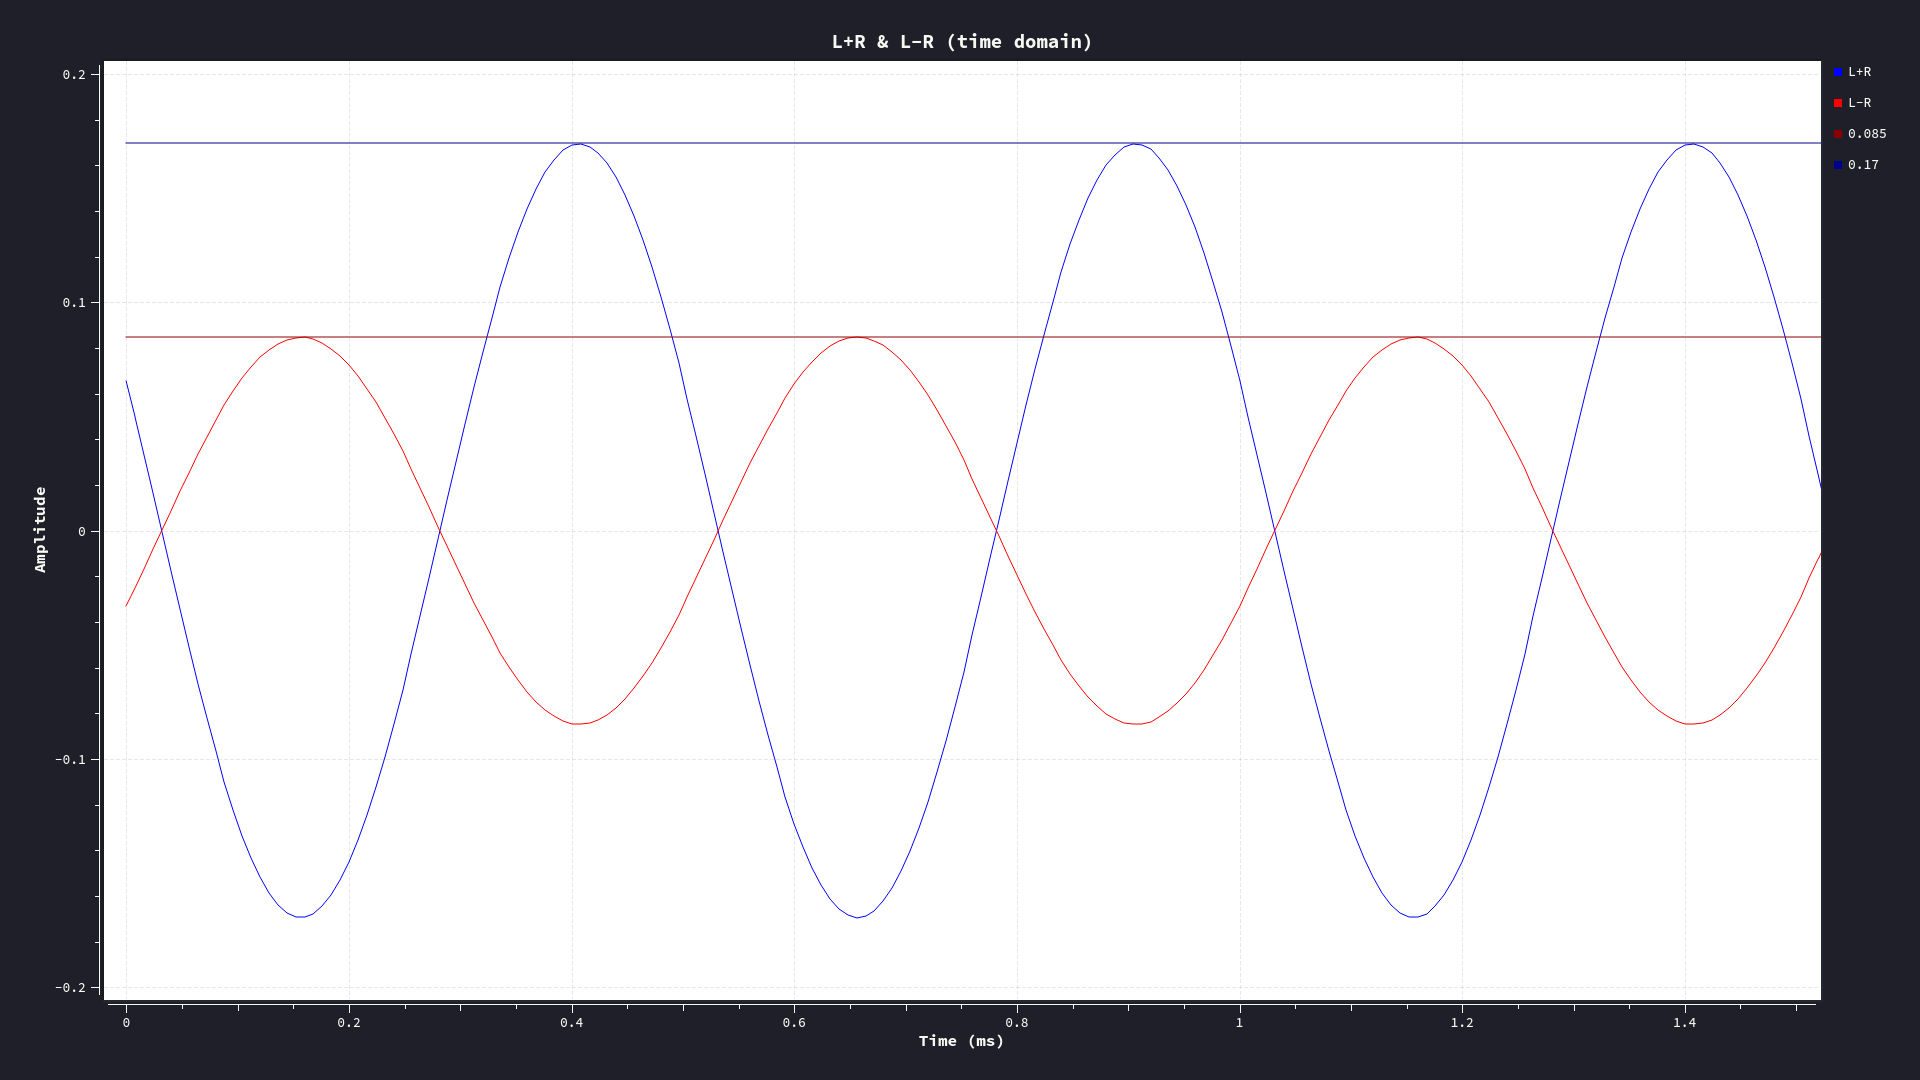
\includegraphics[width=0.8\linewidth]{img/1_2RIGHT.png}
        \caption{RIGHT: visualização de $L+R$ e $L-R$ (domínio \\ do tempo)} 
        \label{fig:ccc} 
        %%\vspace{4ex}
    \end{subfigure}%% 
    \begin{subfigure}[b]{0.5\linewidth}
        \centering
        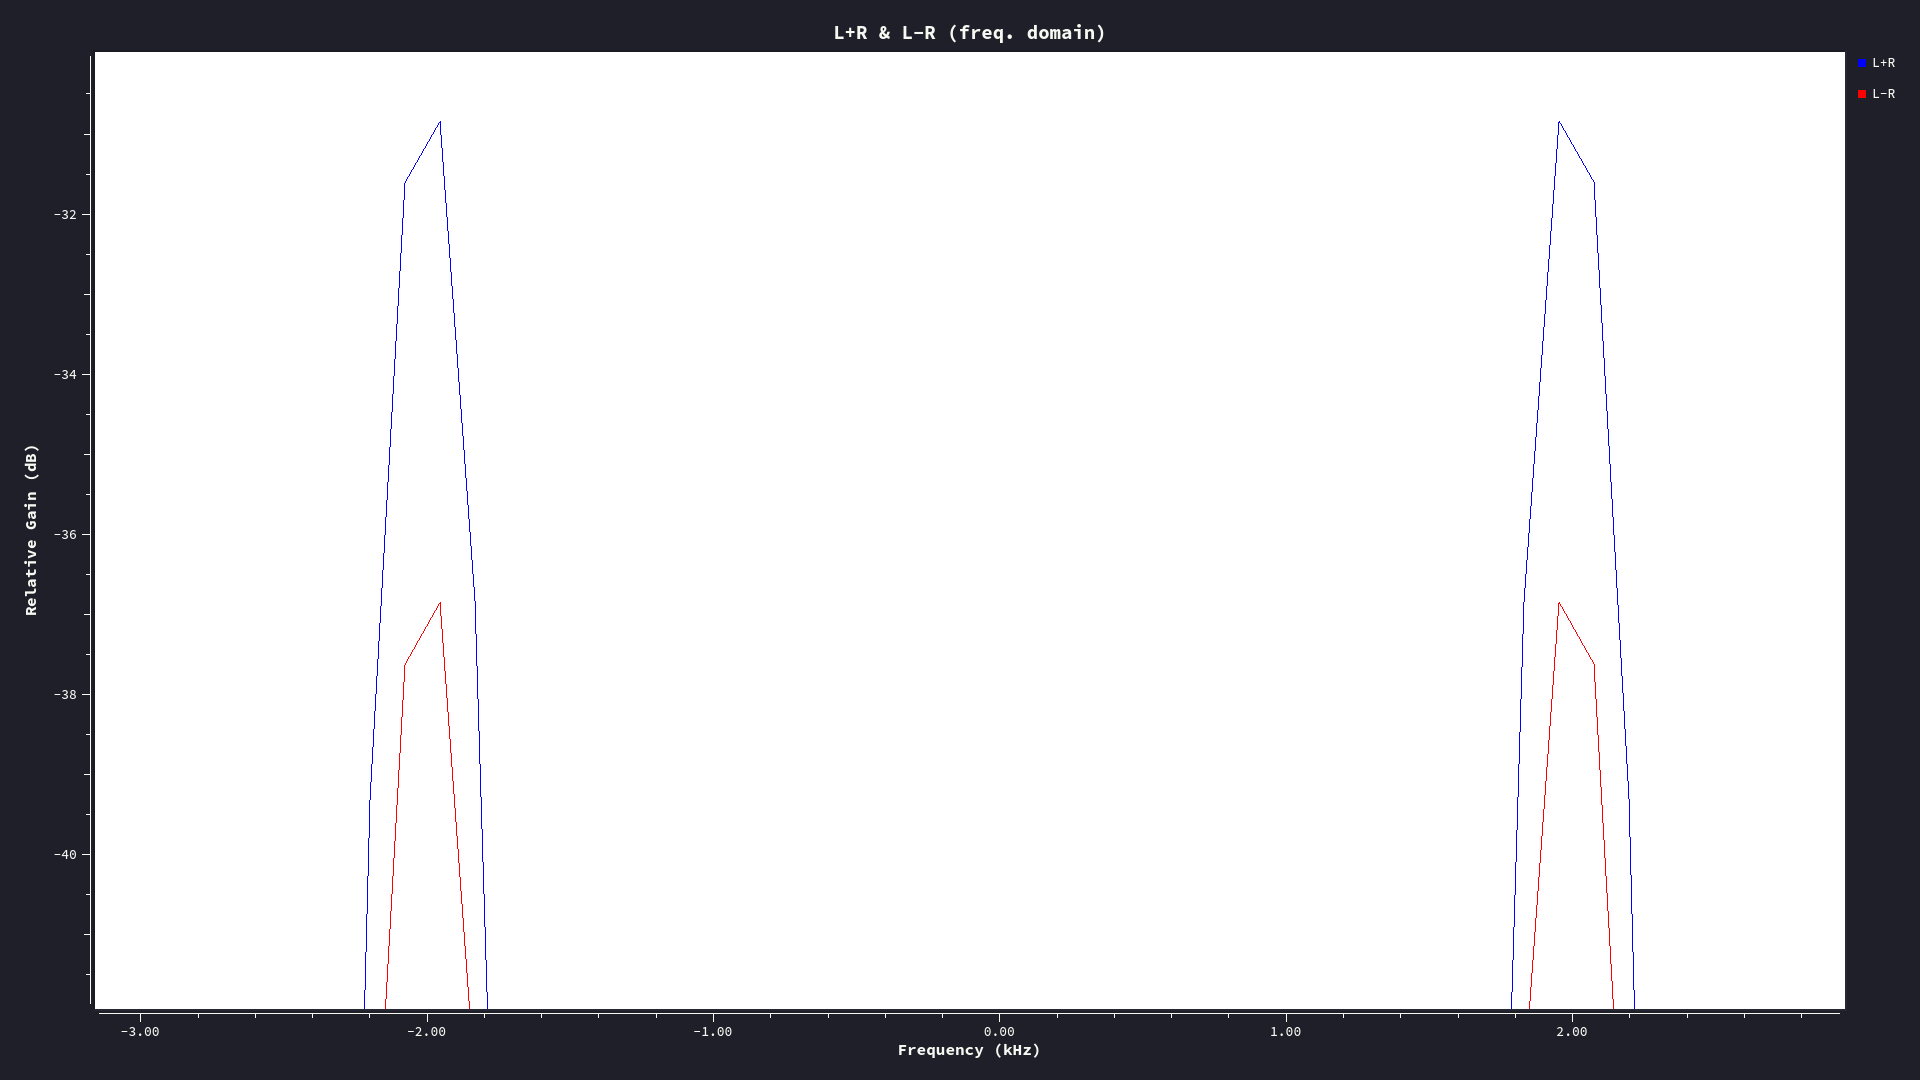
\includegraphics[width=0.8\linewidth]{img/1_2RIGHTdB.png} 
        \caption{RIGHT: visualização de $L+R$ e $L-R$ (domínio \\ da frequência)} 
        \label{fig:ddd} 
        %%\vspace{4ex}
    \end{subfigure} 
    \caption{Visualização do fator de 1/2 extra a compensar.}
    \label{fig:multiplas3}
\end{figure}

Verificando a \hyperref[fig:stereo_spectrum]{Fig. 1}, é aparente que a componente estereofónica DSB-SC dispõe metade do nível de modulação da componente monofónica em cada uma das bandas\cite{transmission_standards_for_fm_sound_broadcasting_at_vhf}. Isto é traduzido nos resultados observados na \hyperref[fig:multiplas3]{Fig. M4}, i.e., no domínio do tempo a componente $L-R$ tem exatamente metade da amplitude de $L+R$, e no domínio da frequência o pico de $L-R$ situa-se a cerca de $6$ dB a baixo\footnotemark[2] do de $L+R$.

\footnotetext[2]{C.A.: $-6$ dB $= 10^{-6/20} \approx 0.5$}

O mesmo raciocínio é aplicado para a obtenção do fator $K$ mencionado anteriormente. 

\begin{figure}[H]
    \centering
    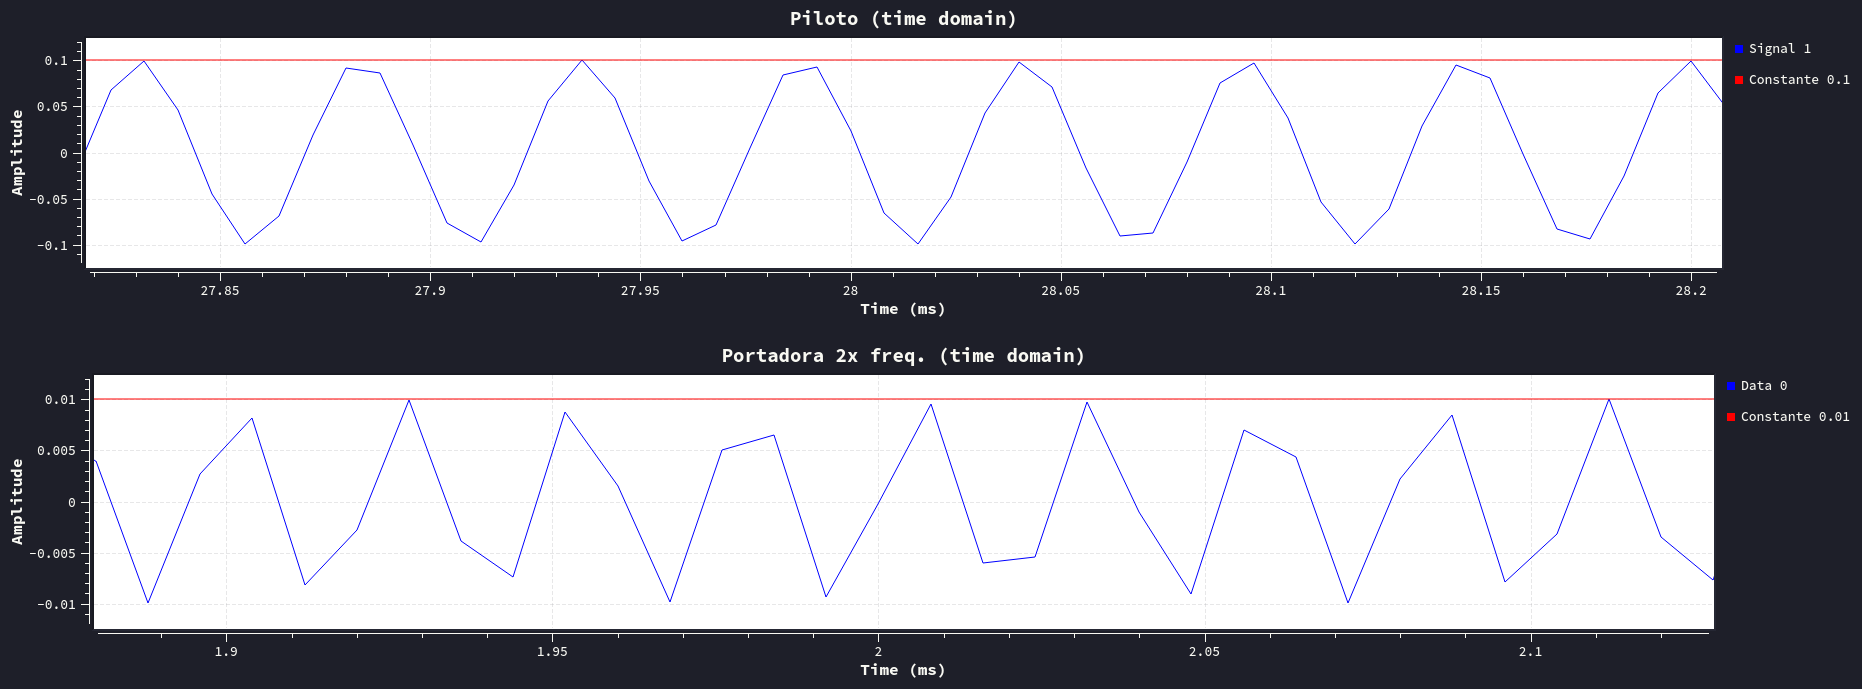
\includegraphics[width = 0.6\linewidth]{img/constanteK.png}
    \caption{Representação no domínio temporal da portadora regenerada (com amplitude $K$) e da respetiva portadora com o dobro da frequência após o processo de duplicação (com aplitude $K^2$).}
    \label{fig:constanteK}
\end{figure}
Deste modo, $K = 0.1$.
$$ \pmb{\therefore} \text{\textbf{Fator total a compensar}}\ = \frac{1}{2}\cdot\frac{1}{2}\cdot 0.01 = \frac{1}{400} \implies \text{\textbf{Ganho}}\ = 400$$

Após estas correções, o sinal $L-R$ está de acordo para o processamento correto\footnotemark[3] no \hyperref[subsec:mod4]{módulo que se sucede}.

\footnotetext[3]{É admitido que os ficheiros de calibração nos traduziram o correto fator de compensação deste ramo para a desmultiplexação de qualquer sinal neste formato. Dado que as emissoras rádio em Lisboa transmitem em formato stereo, mas, maioritariamente com $L=R$, não foi possível realizar mais ensaios que garantissem a robustez deste resultado, visto que dipõem $L-R=0$ efetivamente.}